\documentclass[a4paper, 12pt]{article}
\usepackage{titling}
\usepackage{array}
\usepackage{booktabs}
\usepackage{enumitem}
\usepackage{graphicx}
\usepackage{subfigure}
\usepackage{hyperref}
\usepackage{amssymb}
\usepackage{listings}
\setlength{\heavyrulewidth}{1.5pt}
\setlength{\abovetopsep}{4pt}
\setlength{\parindent}{0pt}
\graphicspath{{.}}

\usepackage[margin=1in]{geometry}

% Must be after geometry
\usepackage{fancyhdr}
\pagestyle{fancy}
\fancyhf{}
\rhead{ECTA Homework XXXXXXXXXXX}
\cfoot{\thepage}

\setlength{\droptitle}{-5em}

\title{Evolutionary Computation Theory and Application  \\
				- Assignment 2: Traveling Salesman Problem -}
\author{Debaraj Barua (9030412), Md Zahiduzzaman (9030432)}

\date{}

\begin{document}

\maketitle

\section{General Remarks }

Please Follow those remarks. Deviating will lead to a reduced score

\begin{itemize}
	\item Lable your axis 
	\item Include a descriptive, not covering legend in your plots
	\item Caption you images with a clear description
	\item Remember to name the file correctly
	\item Make sure that both team members submit the same file, with the same name
	\item Please make sure that all figures and lines are clearly readable
\end{itemize}

\section{Solution}

\begin{table} [h!]
	  \centering
\begin{tabular}{|l|l|}
\hline
\textbf{Parameter} & \textbf{Value}   \\
\hline
Population size & 50 \\
\hline
Crossover Rates &  1\%, 10\%, 50\%, 99\% \\
\hline
Mutation Rates & 1\%, 10\%, 50\%, 99\% \\
\hline
Repetitions & 30 \\
\hline
Generations & 1000 \\
\hline
Average best fitness		 & 72.0185 \\
\hline
\end{tabular}
\caption{80\% mutation rate used for various crossover rate and 80\% crossover rate used for various mutation rate. For 30 repetition, both crossover and mutation rate was set to 99\% }
\label{table:defparams}
\end{table}

\newpage
\section{Results}

\begin{figure}[ht!]
  \centering
  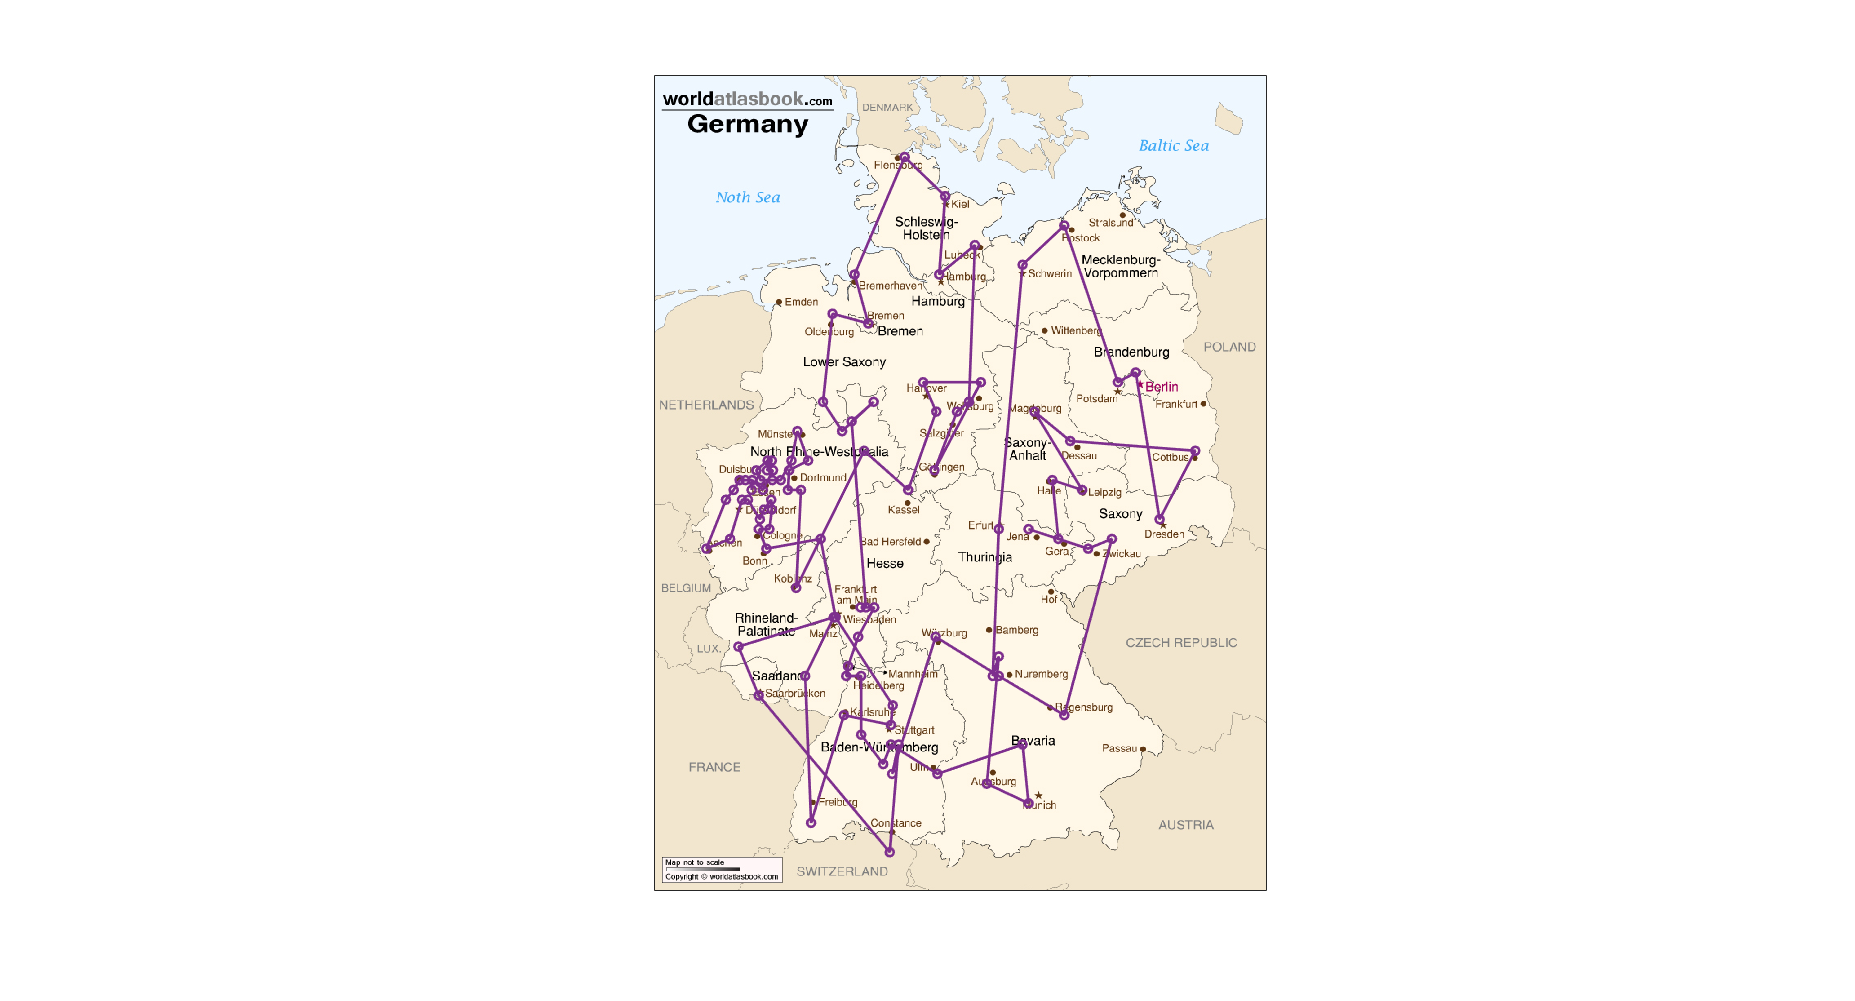
\includegraphics[width=0.7\textwidth]{images/resultmap-mine}
    \caption{Map using 99\% crossover and mutation \label{fig:xxx1}}
\end{figure}

\newpage
\subsection{Different mutation rates}

\begin{figure}[ht!]
	\centering
	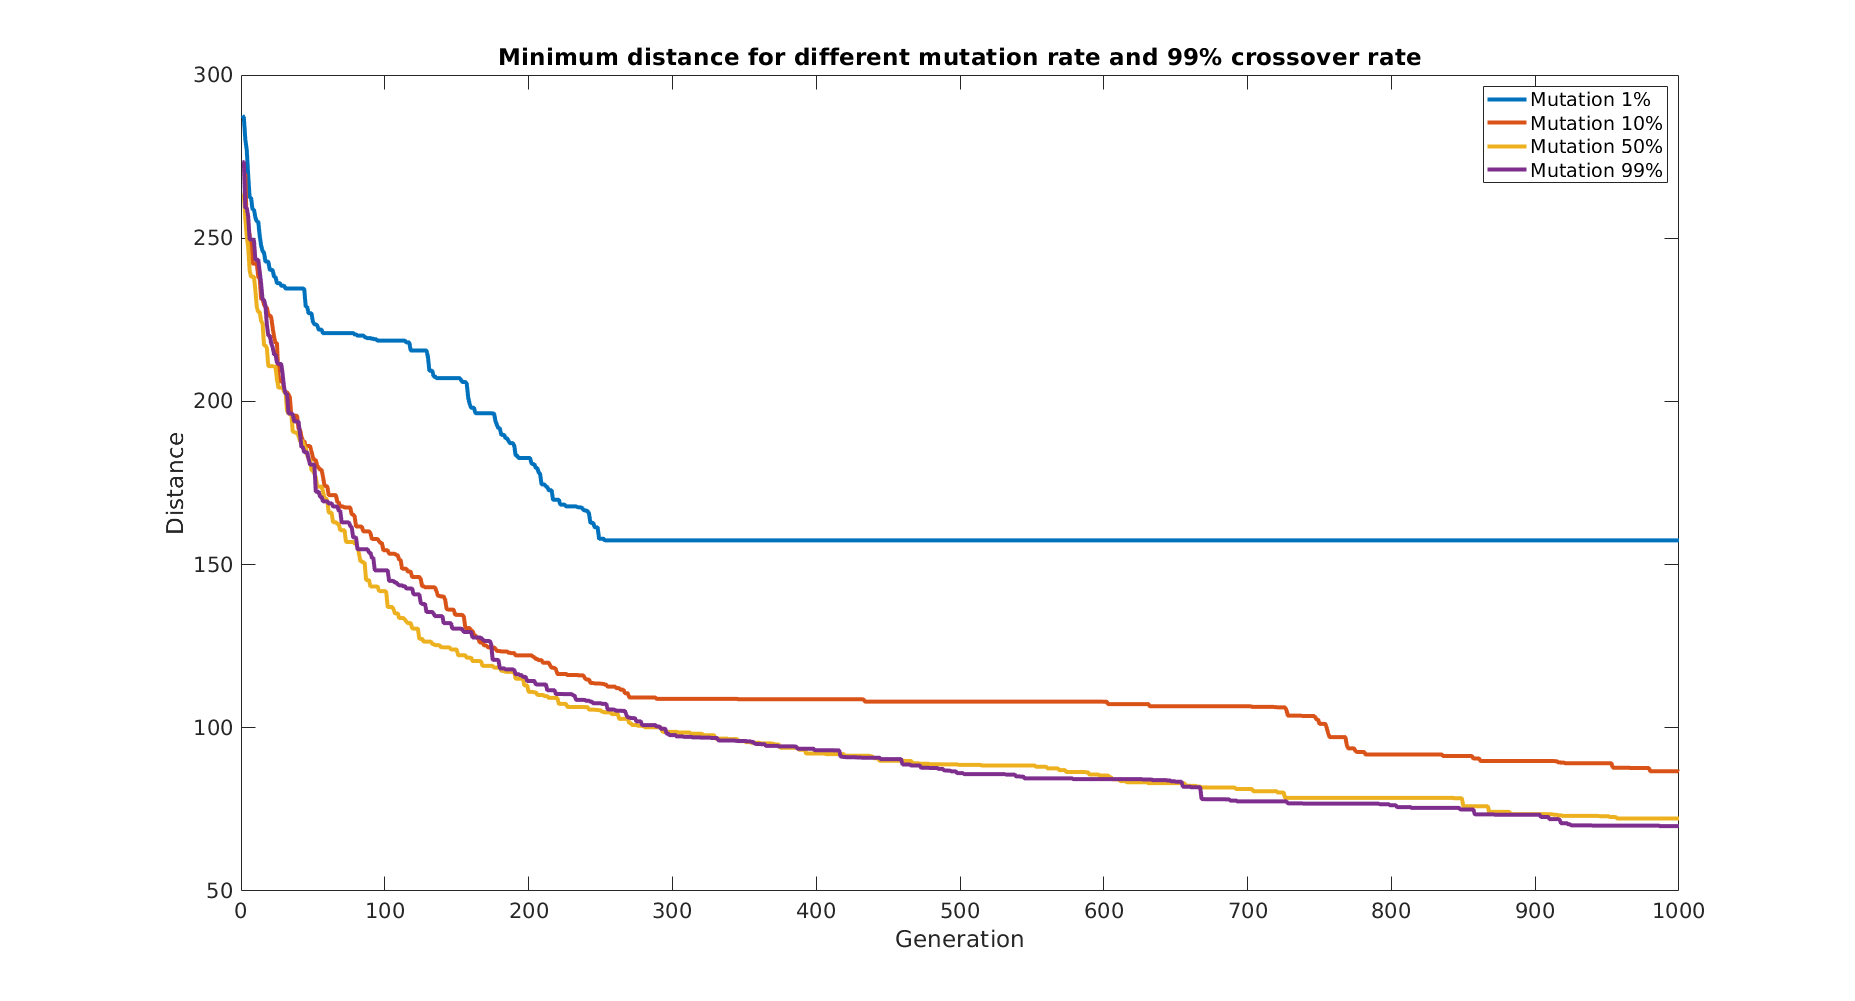
\includegraphics[width=1.0\textwidth]{images/crossfig-mine}
	\caption{Caption describing your plot \label{fig:crossfig}}
\end{figure}

Describe and explain the different mutation rates and how they influence the learning behaviour. Please remember to also focus on why, not only on what.
Also elaborate on the mutation rate you have chosen as best mutation rate.

\newpage

\subsection{Different crossover rates}


\begin{figure}[ht!]
  \centering
  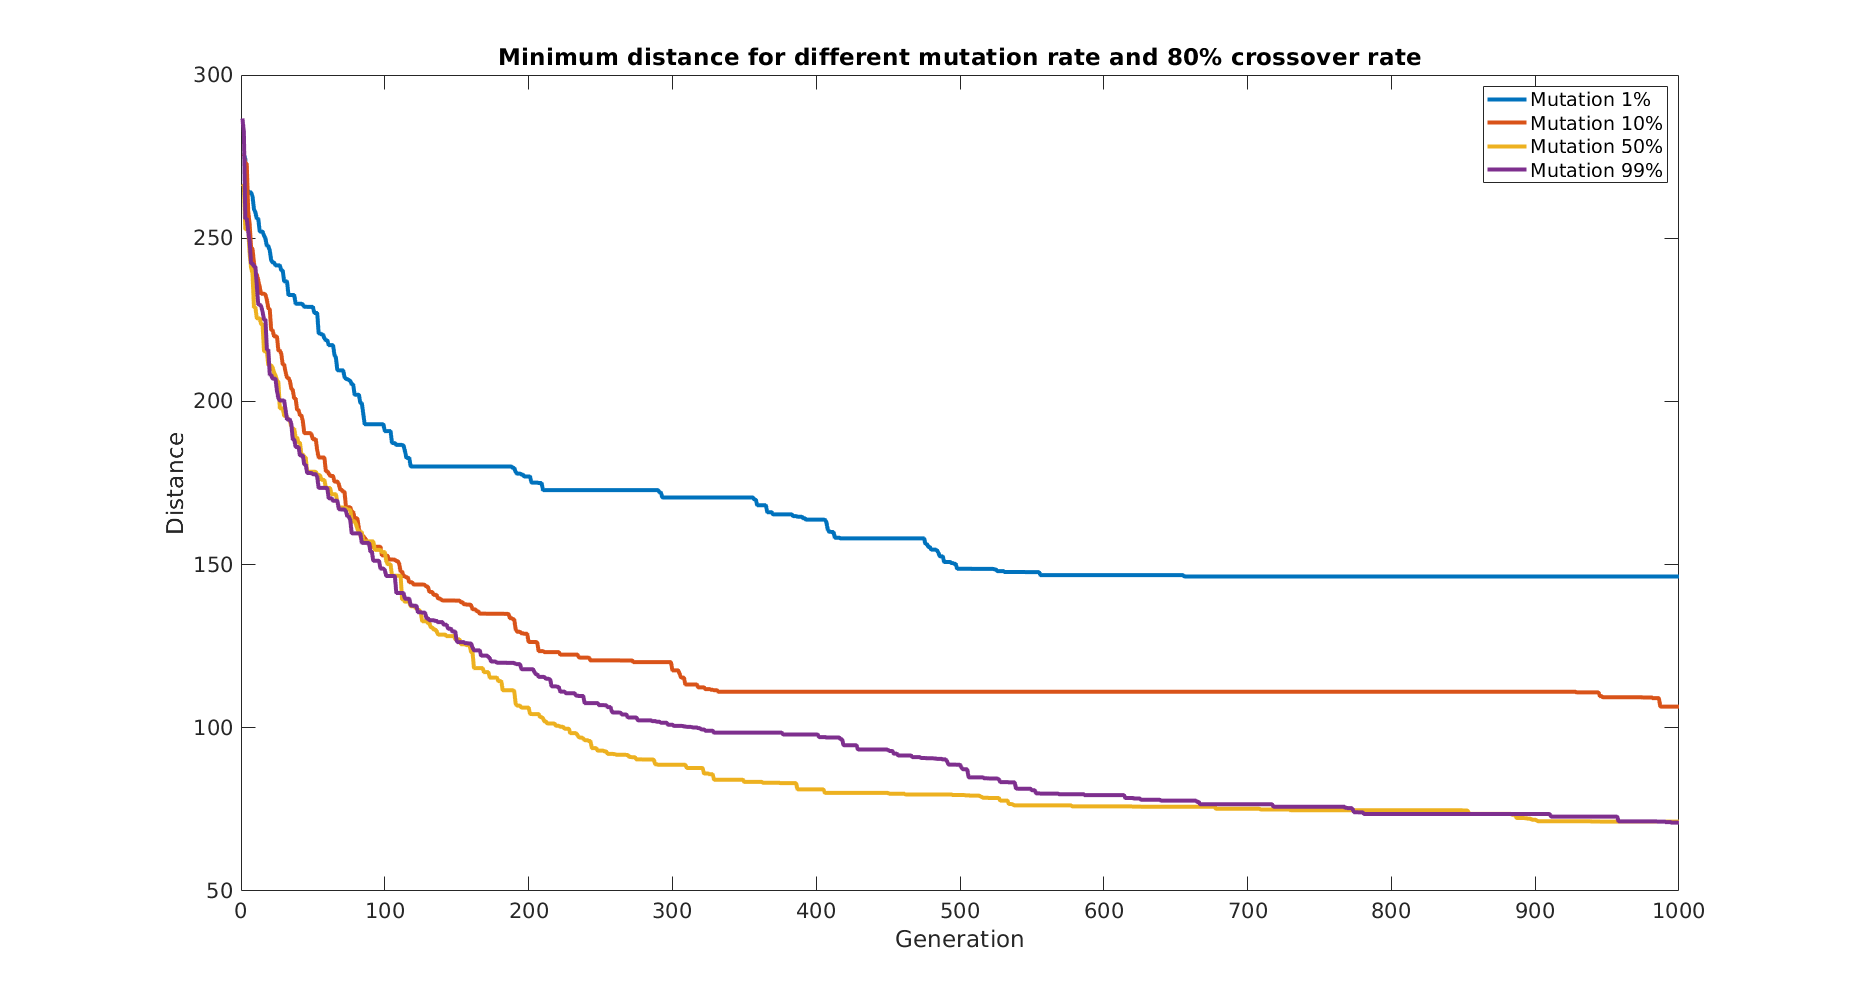
\includegraphics[width=1.0\textwidth]{images/mutfig-mine}
    \caption{Caption describing your plot \label{fig:mutfig}}
\end{figure}

Describe and explain the different crossover rates and how they influence the learning behaviour. Please remember to also focus on why, not only on what.
Also elaborate on the crossover rate you have chosen as best mutation rate.



\end{document}
